\RequirePackage{luatex85,shellesc}
\documentclass[]{resonance}
\usepackage{pgf,tikz}
\usepackage{tikzsymbols}
\usepackage{nameref}
\usepackage{pgfplots}
\usepackage{grffile}
\usepackage{amsmath}
\usepackage{mathtools}
\usepackage{chemfig}
\usepackage{siunitx}
\usepackage{todonotes}
\usepackage{amssymb}
\usetikzlibrary{shapes,backgrounds,calc,arrows,arrows.meta}

\usepackage[acronym]{glossaries}
%\newglossaryentry{CaM}
%{
%    name=Calmodulin,
%    description={Calmodulin}
%}

\newacronym{camkii}{CaMKII}{calcium/calmodulin dependant protein Kinase II}
\newacronym{cam}{CaM}{calmodulin}
\newacronym{psd}{PSD}{Post Synaptic Densitiy}
\newacronym{ca}{Ca\textsuperscript{++}}{calcium}
\newacronym{pp1}{PP1}{protein phophatase 1}
\newacronym{pp2}{PP2}{protein phophatase 2}
\newacronym{cacam}{Ca\textsuperscript{++}/CaM}{calcium/calmodulin complex}
\newacronym{i1p}{I1P}{phosphorylated inhibitor-1}
\newacronym{i1ppp1}{I1P.PP1}{I1P-PP1 complex}
\newacronym{i1}{I1}{inhibitor-1}
\newacronym{can}{CaN}{calcineurin}
\newacronym{pka}{PKA}{protein kinase A}
\newacronym{darpp}{DARPP-32}{a dopamine- and cyclic-AMP regulated neuronal phosphoprotein}
\newacronym{i2}{I2}{inhibitor 2}
\newacronym{sbgn}{SBGN}{System Biology Graphical Notation}
\newacronym{ltp}{LTP}{Long Term Potentiation}
\newacronym{ltd}{LTD}{Long Term Depression}
\newacronym{nmda}{NMDA}{N-methyl-D-asparate}
\newacronym{nmdar}{NMDAR}{N-methyl-D-asparate receptor}
\newacronym{ampa}{AMPA}{$\alpha$-amino-3-hydroxy-5-methyl-4-isoxazolepropionic acid}
\newacronym{mz}{MZ}{Miller and Zhabotinksy}


\newcommand\Fig[1]{\textit{Figure~\ref{#1}}}
\newcommand\TT[1]{\texttt{#1}}

% Title Page
\title{Switches in the brain?} 
\secondTitle{A potential mechanism to long-term memories storage}
\author{Dilawar Singh}
\date{\today}
\begin{document}
\maketitle

\begin{abstract}
    We forget often. But we are also capable of remembering as long
    as we live. This means that our brain is capable of protecting some memories for
    years. This is a remarkable feat given that the \emph{chemical hardware}
    involved in forming biological memories is an extremely hostile place for
    storage.  What are the challenges involved? And what potential mechanisms
    can offer a viable solution? This article explores a major hypothesis that
    molecular switches may be behind our remarkable ability to remember for lifetime.
\end{abstract}

\maketitle
%%\authorIntro is used to place the author's photo and an introduction about the author
%%photo goes into the includegraphics with width=2cm 
%%and a "\\" dividing the text and photo
%%the intro text box is drawn automatically
%%place \authorIntro  just before abstract
% \authorIntro{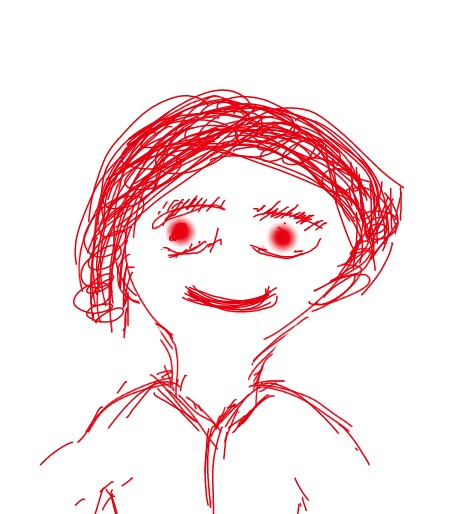
\includegraphics[width=2cm]{dilawar}\\
% }

%%abstract
%%include \monthyear{month year} for month and year of publication in the footer
\monthyear{May 2018}
%%use \artNature for the running head information
\artNature{GENERAL  ARTICLE}

\section{Introduction}\label{sec:intro}

Our brain is made up of roughly 100 billion neurons, joined together with over
100 trillion connections called \textbf{synpase}. Each neuron on average makes
1000 connections.  \leftHighlight{Each neuron, on average, receives roughly 1000
connections from other neurons.} It is now widely accepted that memories are
formed in these connections.

Lets label $n$ of these connections as $s_1, s_2, \ldots s_n$. Any memory can be
represented by a set of connections, for example, my memory of being chased by a
ferocious street dog named \emph{Lalu} (lets call it $M_\text{Lalu}$) is
represented by the set of the synapses $M_\text{Lalu}=(s_{10}, s_{21},
s_{12},\ldots,s_{331})$ i.e. these connections were changed during my troubling encounter with
Lalu. Years later, sometimes I still recall this memory whenever I see a similar
looking dog. 

For most animals, ability to remember and recall such painful encounters with
predators happened in past are most valuable. It helps them in avoiding similar
predators in present and future. I can recall a painful experience as long as
the set of connections in which experience is stored remains \emph{unchanged}.
Can you think of a network made up of neurons and synapse in which you can store
and recall memories? See section "\nameref{sec:hopfield}" for a popular solution.

\begin{figure}[!t] \caption{Memory formation and forgetting. During formation of
    a memory, some synapses become stronger. Longer you can maintain these
connections, longer you can hold on to this memory.  }\label{fig:engram}
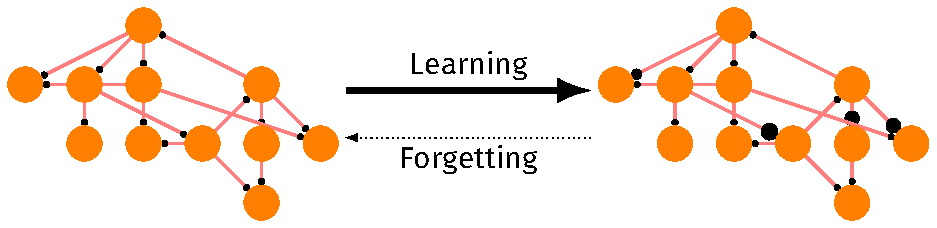
\includegraphics[width=\linewidth]{engram.pdf} \end{figure}

\subsection{Long term memory maintenance}{\label{subsec:ltp_maintenance} 

For $M_\text{Lalu}$ (or any other memory) to remain intact, each of its
component (synapses $s_{10}, s_{21}, s_{12} \ldots$) should also remain intact.
Longer a synapse can keep itself unchanged, better it will be at keeping the
memory. If somehow I can make these synapses to maintain their states for very
long time (rigid synapse), these synapse will not \emph{forget} easily. But this
solution causes another problem. Rigid synapses that do not change will not
participate in any memory formation anymore since learning requires change. On
the other hand, if the synapse is easily changeable (plastic synaspe), it will
be good a learning new experiences but won't be able to retain it for long i.e.
plastic synapse forgets easily. We know that we not only remember for long time,
we are capable of learning quickly.  \leftHighlight{Forgetting and remembering
are two sides of the same coin.} Indeed a good memory system is the one which
learns quickly from new experiences and forgets old information as slowly as
possible.  Forgetting and remembering are the two sides of the same coin.  They
are conflicting demands -- a zero-sum game.  The challenge is to strike a
balance. 

% Hopefield network 
\section{Hopfield network -- associative memory network}\label{sec:hopfield}

Before we continue further, lets familiarize ourselves with one very popular
network made up of neuron like elements in which memories can be stored and
fetched. Memory storage and retrieval is trivially done by a computer. It would
be instructive to compare memory storage in computer and brain. In the computer,
we almost always know the address of every stored memory.  We can access it by
providing the address. The file icon on your desktop is a graphical way of
encoding this addressing scheme. The process is very similar to looking up the
index page in a reference book to find a chapter. Our brain, as far as I know,
does not have such indexing mechanism. 

We usually recall memories when we are provided with \textit{cue}. For example,
when you see some part of of a familiar person in a wedding album -- while rest
of the person may be hidden behind other people -- you could easily identify the
person name, and perhaps some other memories of that person will also be
recalled. A famous class of recurrent neural network often known as Hopefield
network can do just the same as shown in \Fig{fig:hopfield}.

\begin{figure}[!hb]
    \centering
    \caption{Hopfield network with 100 spiking neurons. These \emph{recurrent} configurations have 
        extremely rich dynamics and give rise to interesting brain-like
        computation. \textbf{(B)} 6 patterns (memory) i.e. NCBSXY are stored in this
        network. \textbf{(C)} When a very distorted \textit{cue} is applied to
        the network input, its dynamics converges to one of stored pattern which
        is \emph{closest} to any of the stored pattern.
    }\label{fig:hopfield}
    \includegraphics[width=\linewidth]{./hopfield.pdf}
\end{figure}

How does this recurrent network work is beyond the scope of article. Readers are
encouraged to explore more by themselves. \emph{How well we can explain
biological memory by these network} is an ongoing research area. Though these
networks are extremely successful in accomplishing various \textit{brain-like}
computation (a. la. machine learning), we would like to advise the reader to be
sceptical by noting the following.

\begin{itemize}
    \item  Neurons used in these networks are highly simplified. \textit{Real}
        neurons are not this simple. Even though these simplified neurons
        capture the essential \textit{all-or-none} (electrical spike) way of
        communication and learning by changing synaptic connections, they do
        ignore rich local computations which can be accomplished by branches of
        these neurons (called \textit{dendrites}).
    \item  There is no strong evidence that neurons make such dense recurrent
        connections. However some studies have shown that this is not a
        necessary requirement.
    \item Activity in these networks does not match usually observed activity 
        in the primate brain during memory-recall experiments.
\end{itemize}

\leftHighlight{Despite all their limitations, modeling any phenomenon makes us
think about it concretely.} These network provide us with a framework to
concretely think about the problem of memory storage and its recall. We learn a
great deal about these problem by pointing out the limitations and failure of
these models. Hopfield network has properties which will sound very natural to
us. Can you store as many memories as you like in these networks? No. There is
upper limit. Adding more patterns than this limit cause distortion in memories
i.e. when a cue is given, network no longer fetch the right pattern; and often
fetches a pattern which was not even stored which often resemble some mixture of
stored patterns. When too many memories are stored, they corrupt each other by
mixing up. Also connection weights $w_i$ must not change after storage of memory
else the stored patterns will be corrupted.

After is necessary detour, lets go back to the main theme of the article:
how synapses (the connections between the neurons) maintain their state.

\section{How does a synapse maintain its state?}

Very complex biochemistry plays out during learning that changes the synaptic
strength which surprisingly can be fit into a simple mathematical expression.
Let's assume that synaptic strength $w$ is tightly correlated with some chemical
species $X$ i.e. $w$ changes with $X$. The problem of maintenance of $w$ can now
be rephrased as maintenance of the level or the activity of $X$. For the sake of
simplicity, lets just say variable $X$ (which must be rooted in biochemistry at
synapse) is what control synaptic weight $w$. The problem of ``\emph{synapse
maintaining its state}'' becomes the problem of ``\emph{$X$ maintaining its
state}''.

\begin{figure}[!b]
    \caption{Phosphorylation and deposphorylation of X. P is phosphatase.}\label{fig:model}
    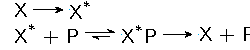
\includegraphics[]{./fig_model.pdf}
\end{figure}

Lets assume that $X$ is converted to its \texttt{ACTIVE} form $X^*$  by adding a
phosphoryl group ($PO_4^{2-}$). The phosphoryl group is removed by a phosphatase
and $X^*$ is turned back into \texttt{INACTIVE} $X$. The phosphorylation and its
counterpart dephosphorylation are a very common motif for controlling various
chemical reactions by \textit{activating} and \textit{inactivating} protein
molecules. If a fraction $f$ of $X$ has been turned into $X^*$, we claim that
synapse strength is $fw_{max}$ where $w_{max}$ is synapse's  strength when all
$X$ has been converted into $X^*$. \textbf{Once $X$ has been turned into $X^*$
during memory formation, how do we make sure that $X^*$ does not turn back
into $X$ (lose memory)}.

Lets mull over a solution to this problem of long term maintenance of $X^*$.
Lets propose that somehow following are true.  \rightHighlight{Can you think of
other set of hypothesis? It must conform to laws of chemistry!}

\begin{enumerate}
    \item \textbf{(Amplification)} $X^*$ \textbf{auto-phosphorylate} itself i.e. \tikz[baseline]{ 
            \node (x) {$X$};
            \node[right=9mm of x] (xp) {$X^*$};
            \draw[-latex] (x) -- (xp);
            \draw[-latex] (xp) edge[out=-120, in=-90] ([xshift=7mm]x);
        }. If we managed to get sufficient $X^*$ somehow, it
        will act as a catalyst to its own production. 
    \item Dephosphorylation of $X^*$ is controlled i.e. 
        phosphatase $P$ has minimal impact on $X^*$.
\end{enumerate} 

Both (1) and (2) helps making $X^*$ highly stable. Good? This means that we have
constructed a very rigid synapse. Recall the \textit{rigid} v/s \textit{pastic}
synpase dilemma discussed previously in section~\ref{sec:intro}. This synapse
will definitely remember for long but it will be impossible for this synapse to
participate in any new learning anymore.

As long as we are in the realm of theory, lets propose a solution to this
problem .  Lets add another reaction say $B+X^*\rightarrow BX \rightarrow B+X$
which deactivates $X^*$ when \textit{need} arise. This adds another layer of
control to already complicated problem i.e. forgetting is now controlled by
another process. This requires another explanation: how does this new mechanism
controlling \textit{forgetting} work. And philosophically, if you care about it,
it violates the principle of \textbf{parsimony} which recommends to pick the
simplest explanation whenever possible. 

\rightHighlight{At synaptic volumes, effect of chemical noise and
\emph{turnover} are strong.} We still have two big problems hiding underneath.
We havn't considered the hardware i.e. synapse in any detail where this
biochemical network suppose to operate. First problem is the chemical noise. For
biochemical system operating in very small volumes, this is a major problem. The
volume of a typical synapse is \SI{1e-20}{\cubic\meter}. At this volume,
\SI{1}{\micro M} concentration is roughly equal to 6 molecules. There are over
200 types of protein molecules in synapse. Indeed, most of these protein
molecules have very low copy number; few tens to few hundreds of molecules of
each protein. Brain is always active. Any chemical noise caused by this
background activity is very likely to turn some molecules of $X$ into $X^*$ and
due to auto-phosphorylation, sooner than later, all of the $X$ will be turned
into $X^*$. We have created a very stable memory of nothing but background
noise. We definitely do not want that!  \marginpar{Show stochastic simulation
here.}.

Second problem is due to \textit{turnover}. Old molecules are constantly
replaced by newly minted molecules. Assume that we have 100 molecules of $X^*$
in synapse and on average, every day one new molecule replaces an old one.
After 50 days, half of the synaptic strength is gone! We must have a mechanism
by which we make sure that the new molecule quickly changes its state according
to the state of synapse i.e. new $X$ becomes $X^*$ if $f$ is large else it
remains $X$. 

We want not only a stable \texttt{ACTIVE} state (all $X$ are $X^*$), but also
chemical noise \emph{not} able to turn $X$ into $X^*$.  We want a switch like
behaviour. If few $X$ are turned into $X^*$ by background noise, we expect them
to be quickly turned back into $X$ by phosphatase. And if during memory
formation, a significant portion of $X$ has been turned into $X^*$ then we
expect that any $X^*$ turned back into $X$ is quickly activated again into
$X^*$.  This system should operates like an switch which does not flip unless
significant force is applied. These are called \textbf{bistable switch}. 

\begin{figure}[b!]
\caption{A hypothetical network which can solve the problem of chemical noise and
    turnover (how?). Activation step has two steps: first slow and then fast. 
    Slow step is to make sure that small fluctuation caused by background noise do not 
    cause system to activate itself. $X^*$ also partially activate $X$ to
    $X^\sim$ to overcome \textit{turnover}.
}\label{fig:model_bistable}
\centering
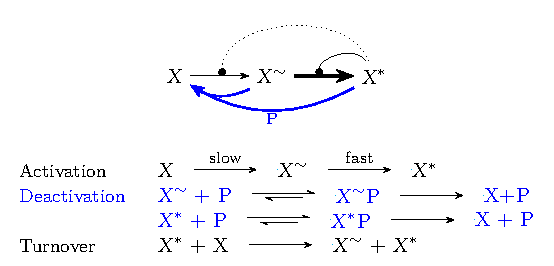
\includegraphics[width=\linewidth]{./fig_model_b.pdf}
\end{figure}


Is there any  proof that bistable systems are even possible? Do they occur at
all in living cells?  Bistability (and its close relative oscillations) are very
common in biology; from cellular level to population levels. So if it won't be
surprising if we find bistable switch at syanpse as well.  \emph{Is there a set
of chemical reactions which forms a bistable switch at synapse?} Various studies
have shown that \gls{camkii} may form a bistable switch at synapse.

\section{Molecular bistable switch at synapse}\label{sec:molecular_switch}

\begin{figure}[ht!]
    \centering
    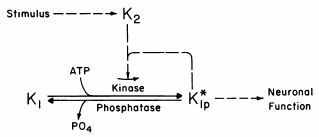
\includegraphics[ ]{./lisman_bistable.png}
    \caption{Reaction in a bistable switch proposed by John Lisman. Modified
        from \cite{lisman1985}. Permission not required for reuse for
        educational purpose.
    }\label{fig:lisman}
\end{figure}

John Lisman hypothesised that a kinase and a phosphatase together
(\Fig{fig:lisman}) can form a bistable switch which is stable against
\emph{turnover}. \gls{camkii} and its phosphatase \gls{pp1} were identified as
the hypothesised kinase and phosphatase. This chemical system had been
extensively studies using compuational models for over last two decades
\cite{sandstorm} and found to be bistable in many computational studies. There
is evidence that \gls{camkii} is bistable \emph{in vitro} conditions. 

\gls{camkii} is known to  play an important role in memory formation.  In
experiments involving mice, deactivating \gls{camkii} in any way has always
resulted in impairment of memory formation and learning. \gls{camkii} molecule
also has many interesting properties which makes it an attractive candidate for
storing memory. 12 to 14 subunits of \gls{camkii} made up one molecules, usually
arranged in dodecameric form. Activation of its first subunit is very slow. Once
a subunit has been activated, it catalyses activation of its neighbours i.e.
\gls{camkii} auto-phosphorylates itself. Moreover fully active \gls{camkii}
holoenzyme can loose an \textit{ACTIVE} subunits which can be picked up by
another holoenzymes. If the gainer holoenzyme was inactive, this holoenzyme
becomes partially active. This process is called subunit-exchange and
\gls{camkii} can spread its activation via it (\Fig{fig:camkii_summary}).

\begin{figure}[b!]
    \caption{ \textbf{(A)} Graphical representation of \gls{camkii} signalling
        pathway. \textbf{(B)} This pathway shows bistable behaviour when synapse
        is receiving background activity. One trajectory is shown for system with 
        15 molecules. \textbf{(C)} Stability of synapse increases exponentially
        with number of \gls{camkii} molecules.
    }\label{fig:camkii_summary}
    \centering
    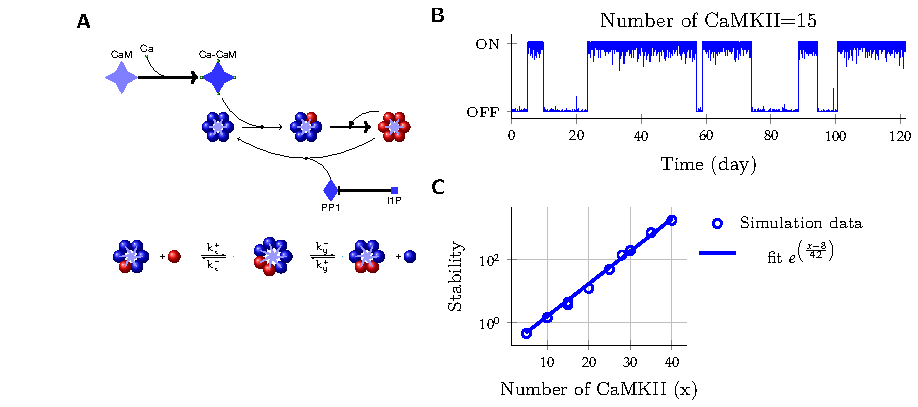
\includegraphics[width=\linewidth]{./resonance_camkii.pdf}
\end{figure}

In our computational study of this pathway, we show that subunit-exchange
improves information retention capacity of \gls{camkii}. We also show that
distributed clusters of \gls{camkii} can form very stable bistable switches; and
can also operate as integrator which is often observed in experiments. In short,
we shows the subunit-exchange makes \gls{camkii} molecule better at retaining
information and it is likely that \gls{camkii} forms bistable switch. To prove
it, one needs to observe single molecule activity in synapse near the membrane
which is very challenging with current technology.

% References section
\section{Conclusion}

In this article, we have discussed why bistable motif is an attractive candidate
for storing biological memories. Most support for this idea has came from
computational studies. To really prove it, we need experimental data supporting
this hypothesis. There is growing experimental evidence that synapse change in
\textit{all-or-none} manner, a finding consistent with this idea. Some studies
claims the changes are graded i.e. synapse changes in step-wise manner much like
a \textbf{multistable} synapse. A multistable synapse is a ensemble of many
bistable components. Whether \gls{camkii} is bistable in synapse (or in some
special confined part of it) is still an open question. So far there is no
concrete evidence that it is. There could be other still unknown mechanisms which can
give rise to bistability. Given that bistable motif is a widespread theme in
biology, it is reasonable to believe that there are indeed switches in our brain
-- much like flip-flops in digital memory -- which keeps our memories safe from
the onslaught of time and noise.

\begin{thebibliography}{99} 
    \bibitem{lisman1985} 
    Lisman J. E., 
    \textit{A mechanism for memory storage insensitive to molecular turnover: a
    bistable autophosphorylating kinase}. 
    Proc. Natl. Acad. Sci. USA, May 1985

    \bibitem{koch1999}
    Christof Koch
    \textit{Biophysics of computations}.
    Oxford University Press, 1999.

    \bibitem{sandstorm} 
    Malin Sandstorm,
    \textit{Models of CaMKII activation},
    Master Thesis, Royal Institute Of Technology Sweden 


\end{thebibliography}

\end{document}
